\documentclass[10pt,a4paper]{article}
\usepackage[utf8]{inputenc} 
\usepackage[spanish]{babel}
\usepackage{a4wide}
\usepackage{float}
\usepackage{caratula}

\begin{document}

\titulo{Trabajo Práctico}
\subtitulo{SLS: Un simple lenguaje de scripting}

\fecha{\today}

\materia{Teoría de Lenguajes}
\grupo{Los Libres de Contexto}

\integrante{Castro, Alan}{356/10}{alancastro90@gmail.com}
\integrante{Bonomi, Cyntia}{134/03}{cyntiab83@gmail.com}
\integrante{Izcovich, Sabrina}{550/11}{sizcovich@gmail.com}

\maketitle

\tableofcontents

\newpage

\section{Gramática}

En lo que sigue, presentamos la gramática utilizada para la realización del parser:\\

S' $\rightarrow$ program \\
program $\rightarrow$ list\_sentencies \\
list\_sentencies $\rightarrow$ COMMENT a \\
list\_sentencies $\rightarrow$ sentence a \\
a $\rightarrow$ list\_sentencies \\
a $\rightarrow$ $\lambda$ \\
sentence $\rightarrow$ e SEMICOLON \\
sentence $\rightarrow$ WHILE LPAREN expression RPAREN keys \\
sentence $\rightarrow$ IF LPAREN expression RPAREN keys possibleelse \\
sentence $\rightarrow$ FOR LPAREN assignationorlambda SEMICOLON expression SEMICOLON advancefor RPAREN keys \\
sentence $\rightarrow$ DO keys\_do WHILE LPAREN expression RPAREN SEMICOLON \\
sentence $\rightarrow$ function SEMICOLON \\
sentence $\rightarrow$ RETURN expression \\
possibleelse $\rightarrow$ ELSE keys \\
possibleelse $\rightarrow$ $\lambda$ \\
e $\rightarrow$ advance \\
e $\rightarrow$ assignation \\
comment\_list $\rightarrow$ COMMENT comment\_list \\
comment\_list $\rightarrow$ $\lambda$ \\
keys\_do $\rightarrow$ comment\_list sentence \\
keys\_do $\rightarrow$ LKEY list\_sentencies RKEY \\
keys $\rightarrow$ comment\_list sentence \\
keys $\rightarrow$ LKEY list\_sentencies RKEY \\
assignationorlambda $\rightarrow$ assignation \\
assignationorlambda $\rightarrow$ $\lambda$ \\
assignation $\rightarrow$ VAR b \\
b $\rightarrow$ LBRACKET expression RBRACKET ASSIGN expression \\
b $\rightarrow$ ASSIGN expression \\
b $\rightarrow$ COLON expression \\
advancefor $\rightarrow$ advance \\
advancefor $\rightarrow$ assignationorlambda \\
advance $\rightarrow$ VAR LBRACKET expression RBRACKET c \\
advance $\rightarrow$ VAR LBRACKET expression RBRACKET d \\
advance $\rightarrow$ VAR c \\
advance $\rightarrow$ VAR d \\
advance $\rightarrow$ d VAR \\
advance $\rightarrow$ d VAR LBRACKET expression RBRACKET \\
d $\rightarrow$ INCREMENT \\
c $\rightarrow$ PLUSEQUAL expression \\
d $\rightarrow$ DECREMENT \\
c $\rightarrow$ MINEQUAL expression \\
c $\rightarrow$ MULEQUAL expression \\
c $\rightarrow$ DIVEQUAL expression \\
value $\rightarrow$ MINUS LPAREN num RPAREN \\
value $\rightarrow$ MINUS LPAREN function\_with\_return RPAREN \\
value $\rightarrow$ MINUS LPAREN VAR s RPAREN \\
value $\rightarrow$ MINUS function\_with\_return \\
value $\rightarrow$ MINUS VAR s \\
value $\rightarrow$ STRING \\
value $\rightarrow$ bool \\
value $\rightarrow$ num \\
value $\rightarrow$ function\_with\_return \\
s $\rightarrow$ LBRACKET expression RBRACKET s \\
s $\rightarrow$ $\lambda$ \\
value $\rightarrow$ VAR s \\
value $\rightarrow$ LBRACKET expression list\_values RBRACKET \\
list\_registers $\rightarrow$ VAR COLON expression l \\
l $\rightarrow$ COMMA list\_registers \\
l $\rightarrow$ $\lambda$ \\
list\_values $\rightarrow$ COMMA expression list\_values \\
list\_values $\rightarrow$ $\lambda$ \\
value $\rightarrow$ LKEY list\_registers RKEY \\
expression $\rightarrow$ t QUESTIONMARK expression COLON expression \\
expression $\rightarrow$ t \\
t $\rightarrow$ term OR t \\
t $\rightarrow$ term \\
term $\rightarrow$ factor AND term \\
term $\rightarrow$ factor \\
factor $\rightarrow$ factor POW x \\
factor $\rightarrow$ x \\
x $\rightarrow$ y EQUAL x \\
x $\rightarrow$ y UNEQUAL x \\
x $\rightarrow$ y \\
y $\rightarrow$ z GREATER y \\
y $\rightarrow$ z LESS y \\
y $\rightarrow$ z \\
z $\rightarrow$ z PLUS h \\
z $\rightarrow$ z MINUS h \\
z $\rightarrow$ h \\
h $\rightarrow$ h TIMES r \\
h $\rightarrow$ h DIVIDE r \\
h $\rightarrow$ h MODULE r \\
h $\rightarrow$ r \\
r $\rightarrow$ NOT value \\
r $\rightarrow$ NOT LPAREN expression RPAREN \\
r $\rightarrow$ value \\
r $\rightarrow$ LPAREN expression RPAREN \\
function $\rightarrow$ function\_with\_return \\
function $\rightarrow$ PRINT LPAREN expression RPAREN \\
function\_with\_return $\rightarrow$ MULTIPLICACIONESCALAR LPAREN param\_me RPAREN \\
function\_with\_return $\rightarrow$ CAPITALIZAR LPAREN expression RPAREN \\
function\_with\_return $\rightarrow$ COLINEALES LPAREN expression COMMA expression RPAREN \\
function\_with\_return $\rightarrow$ LENGTH LPAREN expression RPAREN \\
param\_me $\rightarrow$ expression COMMA expression n \\
n $\rightarrow$ COMMA expression \\
n $\rightarrow$ $\lambda$ \\
num $\rightarrow$ DECIMAL \\
num $\rightarrow$ NATURAL \\
num $\rightarrow$ NEGATIVO \\
bool $\rightarrow$ TRUE \\
bool $\rightarrow$ FALSE \\

\newpage
\subsection{Atributos}

Dada la limitación de \textit{PLY} para manejar atributos heredados, todos nuestros atributos son sintetizados.\\

Los atributos con los que contamos son:
\begin{itemize}
\item \textbf{NoTerminal.value}/\textbf{Terminal.value}: Consiste en el valor asociado al terminal/no terminal.
\item \textbf{NoTerminal.type}/\textbf{Terminal.type}: Representa el tipo del terminal/no terminal. Se presenta como \textbf{\{"tipo": tipo,"tipoInterno": tipo\}}, donde el $tipo$ consiste en el tipo básico del terminal/no terminal en cuestión, y el $tipoInterno$ consiste en el tipo de los elementos en el caso en el que se trate de un arreglo.
\item \textbf{NoTerminal.isTrue}: \textit{bool}. Almacena el dato de si el booleano pasado por parámetro en multiplicacionEscalar es o no verdadero.
\item \textbf{NoTerminal.stringInterno}: \textit{string}. Sirve para obtener el tipo de un elemento de un array o el tipo de un atributo de un registro.
\item \textbf{NoTerminal.isPlusEqual}: \textit{bool}. Posee la información de si el operador aplicado es +=.
\item \textbf{NoTerminal.line}: \textit{int}. Posee la información de la línea en la que se encuentra la sentencia en el texto original.
\item \textbf{NoTerminal.dict}: \textit{dict}. Consiste en el diccionario de tipos de los elementos de un arreglo que luego se le asignará al tipoInterno.
\end{itemize}

\section{Ejemplo de la Gramática de Atributos}

\begin{figure}[H]
\begin{center}
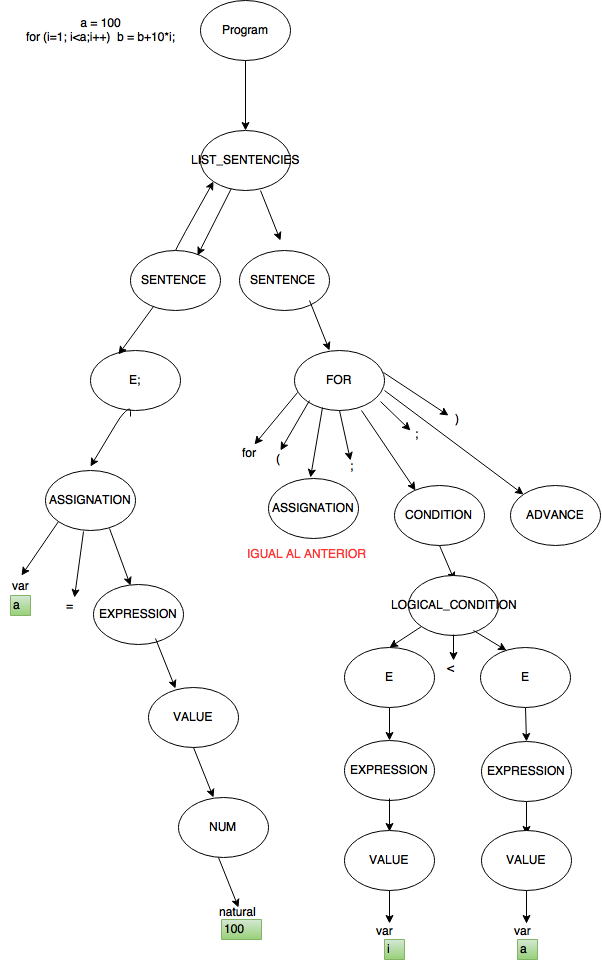
\includegraphics[scale=0.7]{imgs/ejemploGramatica.png}
\end{center}
\end{figure}

En el diagrama anterior, se pueden observar las derivaciones de una parte del programa presentado a modo de ejemplo.

\section{Conflicto del ELSE}
Nuestra gramática presenta un conflicto de tipo shift/reduce en el \textbf{ELSE}. Éste se puede ver en el siguiente caso:

\begin{verbatim}
sentence -> IF LPAREN expression RPAREN keys . possibleelse
possibleelse -> . ELSE keys
possibleelse -> .
\end{verbatim}

Consiste en un conflicto introducido por la ambigüedad que presenta la gramática para este caso, en el que el parser no sabe si debe shiftear o reducir. Sin embargo, toma la decisión correcta, es decir, si en la entrada tiene un ELSE shiftea, de lo contrario reduce.

Es posible desambigüar la gramática (puede verse en la sección 4.3.2 \textit{Eliminación de la ambigüedad} en $Referencia[1]$ replicando todas las producciones para el caso del ELSE por un lado, y el caso sin el ELSE por el otro, sin embargo, al ser un conflicto permitido por la cátedra, usamos la forma ambigüa.

\section{Descripción}

\subsection{Operaciones no permitidas}

Nuestra gramática no permite las expresiones de tipo array[i].atributo para registros dentro de algun arreglo.
Por ejemplo, si tenemos

\begin{verbatim}
usuarios = [{nombre:"Mr.X", edad:10}, {nombre:"Al", edad:50}];
\end{verbatim}

no permitimos la operación 
\begin{verbatim}
edad = usuarios[i].edad;
\end{verbatim}
Realizar esa operación requiere un cambio en la gramática a la hora de ``generar'' variables que no contemplamos desde un principio debido a la decisión de utilizar tipos básicos para los registros.

Por este motivo, los tests $regs.i$ y $all.i$ no funcionan en su integridad, sino que funcionan quitando las líneas que poseen operaciones de la índole de la presentada en el ejemplo anterior. 

\subsection{Estructura de tipos}

Para el resguardo de las variables con sus atributos utilizamos un diccionario \textit{table} donde se almacena la siguiente información: 
\begin{itemize}
\item \textbf{Registros:}
\begin{verbatim}
nombreVariable: { "tipo": "register", "tipoInterno": unTipo}
\end{verbatim}
\item \textbf{Arreglos:}
\begin{verbatim}
nombreVariable: { "tipo": "array", "tipoInterno": unTipo}
\end{verbatim}

\item \textbf{Tipos básicos (booleanos, strings, naturales, negativos, decimales):}
\begin{verbatim}
nombreVariable: { "tipo": "tipoBasico", "tipoInterno": None}
\end{verbatim}
\end{itemize}
\textbf{Ejemplos:}
\begin{itemize}
\item 
\begin{verbatim}
numeros = [[1, 2], [3]]
\end{verbatim}
\textbf{Datos en la tabla de tipos:}
\begin{verbatim}
{"numeros": 
    {"tipo": "array", "tipoInterno": 
        {"tipo": "array","tipoInterno":
            {"tipo": "natural", "tipoInterno":None}
        }
    }
}
\end{verbatim}
\item 
\begin{verbatim}
persona = { nombre : "juan", edad : 25 , padres: { mama: "maria", papa: "luis"}}
\end{verbatim}
\textbf{Datos en la tabla de tipos:}
\begin{verbatim}
{"persona": 
    {"tipo" : "register",
       "tipoInterno":{"nombre":{"tipo":"string","tipoInterno": None},
                       "edad":  {"tipo":"natural","tipoInterno": None},
                       "padres":{"tipo":"register","tipoInterno":
                                      {"mama": {"tipo":"string", "tipoInterno": None},
                                       "papa": {"tipo":"string", "tipoInterno": None}
                                       }
                                }
                     }
 }
\end{verbatim}
\end{itemize}
\section{Compilación y ejecución}
Para compilar nuestro trabajo práctico y ejecutarlo, alcanza con correr en la consola el siguiente comando:
\textbf{./SLSparser.py -o archivoSalida -c archivoEntrada} 
Los parámetros son opcionales. Por default, la entrada y salida son la consola en el caso en el que no se especifique alguno de los archivos.
Al pasar un programa por stdin, la finalización del mismo se indica a través del comando \textit{ctrl+d}

\section{Casos de prueba}
Los casos de prueba utilizados fueron los del enunciado y los tests provistos, con los que nos aseguramos que se devolviera un error en cuanto la sintáxis no era correcta. Dadas algunas decisiones mencionadas anteriormente, no todos los tests de la cátedra son aceptados por nuestra gramática (regs.i y all.i).
\section{Conclusión}
Podemos concluir que resulta muy complicado realizar una gramática de tal dimensión sin tener problemas de ambigüedad y que es necesario definir de antemano la precedencia de cada operador antes de comenzar el código. A pesar de ello, PLY es una excelente herramienta para dicho fin dado que resuelve los conflictos solucionándole muchos problemas al programador.

\section{Referencias}
\begin{itemize}
\item \textbf{Aho, Sethi, Ullman}, \textit{Compilers: Principles, Techniques, and Tools}, Addison-Wesley, 1986. ISBN 0-201-10088-6

\item \textbf{Python Lex-Yacc} \textit{http://www.dabeaz.com/ply/}
\end{itemize}

\end{document}
